\section{Gestión de proyectos}

\subsection{Autoevaluación}
\paragraph{}
En esta sección se han cumplido los objetivos correspondientes al 10.

\subsection{Introducción}
\paragraph{}
La organización de las tareas dentro de un equipo es esencial para lograr los objetivos con éxito. Odoo ofrece una herramienta fácil, visual e intuitiva para gestionar las diferentes tareas de cada equipo de trabajo dentro de nuestra empresa.

\subsection{Metodología}
\paragraph{}
Para utilizar este módulo, primero debemos instalarlo. Al igual que el resto de módulos, nos dirigimos a la pantalla de las aplicaciones y buscamos e instalamos el módulo \textit{Proyecto}. Una vez instalado, podemos abrirlo en la esquina superior izquierda. Se mostrará la ventana principal en la cual aparecerán nuestros proyectos, al ser la primera vez que se abre se encuentra vacía. Se debe pulsar en el botón \textit{Nuevo}, rellenar el formulario con el nombre del proyecto deseado y pulsar el botón de crear. Se abrirá automáticamente la página del proyecto recién creado. Lo primero que debemos hacer para comenzar a gestionar nuestro proyecto es crear las columnas para clasificar las tareas. En nuestro caso, hemos decidido dividirlas en tres estados: \textit{Pendiente}, \textit{En proceso} y \textit{Hecho}. Para crear las columnas, se pulsa en el botón \textit{+ Etapa} y se escribe el nombre. Por último, se debe realizar una configuración previa para poder utilizarlo para gestionar nuestras tareas. Nos dirigimos a la ventana de ajustes y seleccionamos \textit{Proyecto}. Aparecerán varias opciones que podemos añadir, en nuestro caso, hemos decidido utilizar la \textit{Dependencia de tareas}. Esta opción permite determinar el orden de las tareas y bloquearlas hasta que se hayan completado con éxito otras tareas.
\paragraph{}
Tras realizar la configuración pertinente al módulo, podemos hacer uso de él. En el proyecto deseado se crean las tareas y se colocan en la columna que corresponda. En un primer momento, las tareas se encontrarán en el estado \textit{Pendiente} y según vaya avanzando el tiempo, las tareas se irán cambiando de columna. Las tareas pueden ser asignadas a miembros del equipo, pueden tener una fecha límite, etiquetas, subtareas, bloqueos y pueden ser prioritarias. Todas estas configuraciones se hacen seleccionando la tarea y modificando los campos deseados. Estas configuraciones nos facilitan la organización de las tareas y tener muy claro de forma visual qué es lo que hay que hacer, en qué tiempo, quién está realizando cada tarea y el flujo de trabajo del equipo.

\subsection{Resultados y análisis}
\paragraph{}
Como hemos mencionado previamente, es fundamental organizar las tareas para cumplir con el plazo y realizar todas las tareas. Durante la realización del análisis de Odoo y la creación de la memoria, hemos decidido utilizar este módulo, consiguiendo evaluarlo de la mejor forma posible y obteniendo las ventajas del módulo para nuestro proyecto.
\paragraph{}
Hemos decidido organizar el tablero con tres columnas: \textit{Pendiente}, \textit{En proceso} y \textit{Hecho}. La primera son aquellas tareas que no se han empezado a realizar, en la segunda se encuentran las tareas que se están realizando y en la última las tareas que han sido completadas. Cada tarea, a su vez, está dividida en cuatro subtareas, cada subtarea corresponde con los objetivos marcados, obtener un cinco, un siete, un ocho o un diez. Todas las tareas tienen como fecha límite el día previo a la entrega, salvo la última tarea (\textit{Memoria final}) que tiene como fecha límite el día de la entrega. Además, se han etiquetado según el grado de dificultad que hemos considerado, pudiendo ser: \textit{Hard}, \textit{Medium} e \textit{Easy}. En nuestro caso, no hemos asignado las tareas a ningún miembro ya que desde el comienzo del proyecto hemos decidido realizar todas las tareas de forma conjunta. Es cierto que al tener que trabajar de forma simultánea nos puede costar más tiempo, sin embargo, consideramos que de esta forma ambos integrantes del equipo aprendemos todas las funcionalidades que nos ofrece este ERP y nos ayudamos mutuamente. También hemos decidido que la tarea más prioritaria es la \textit{Memoria final}, ya que es la tarea a entregar y que hay que cumplir con el plazo. Además, esta tarea tiene una dependencia con las otras tareas. No se puede realizar hasta que todas las tareas de los módulos se hayan completado.

\begin{figure}[h]
    \centering
    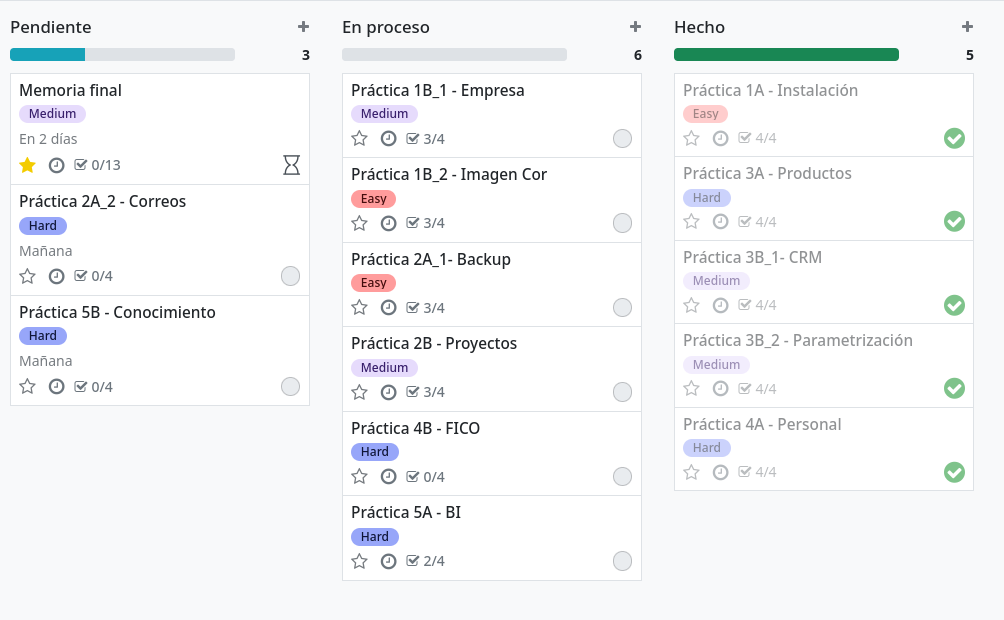
\includegraphics[width=1\linewidth]{proyecto.png}
    \caption{Vista Kanban de nuestro proyecto}
\end{figure}

\begin{figure}[h]
    \centering
    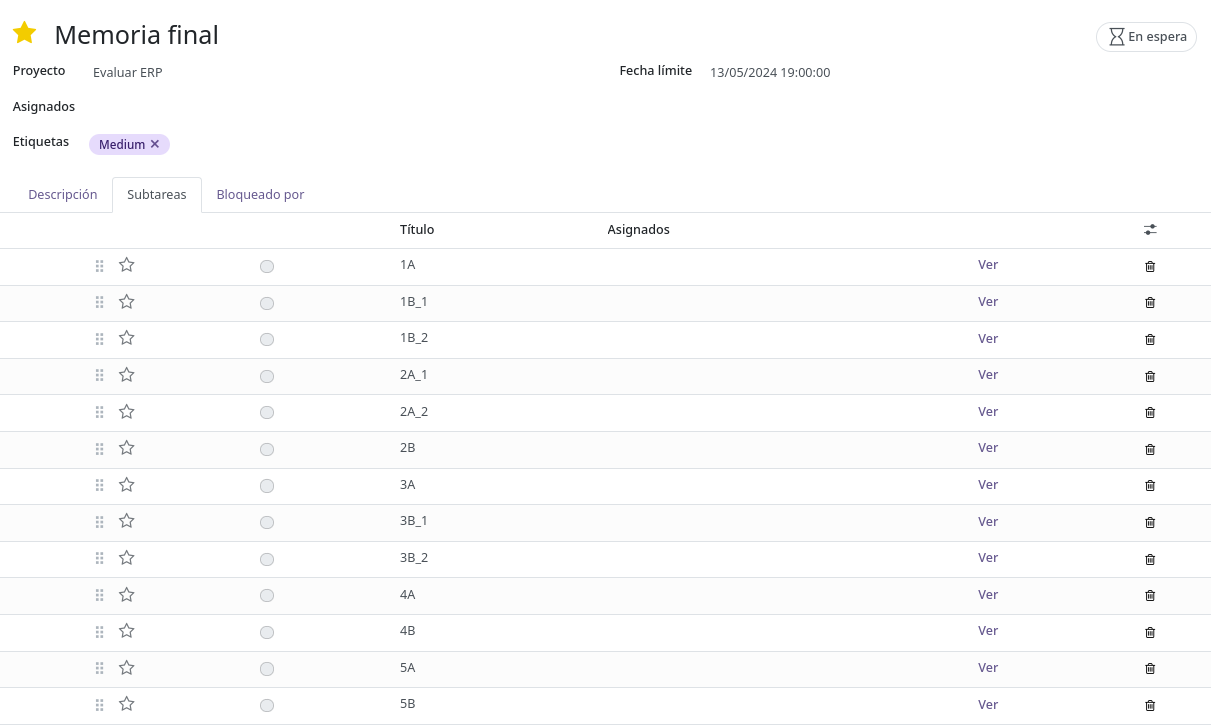
\includegraphics[width=0.75\linewidth]{tareaMemoria.png}
    \caption{Vista de una tarea}
\end{figure}
\paragraph{}
El flujo de trabajo de un equipo de trabajo que tiene un líder y trabajadores es diferente al que nosotros hemos realizado. Este flujo se basaría en que el líder define las tareas y las añade al tablero. Añade los datos pertinentes a la tarea y se la asigna a un miembro del equipo. Esta persona, cuando vea que se le ha asignado una tarea, la moverá a la columna de \textit{En proceso} y se pondrá a realizarla. Una vez que la haya acabado, cambiará el estado de la tarea a \textit{Hecho} y esperará a que se le asigne una nueva tarea. El flujo de trabajo descrito se ve reflejado en el diagrama BPMN (ver Figura \ref{fig:BMMN_trabajo}). 

\begin{figure}[h]
    \centering
    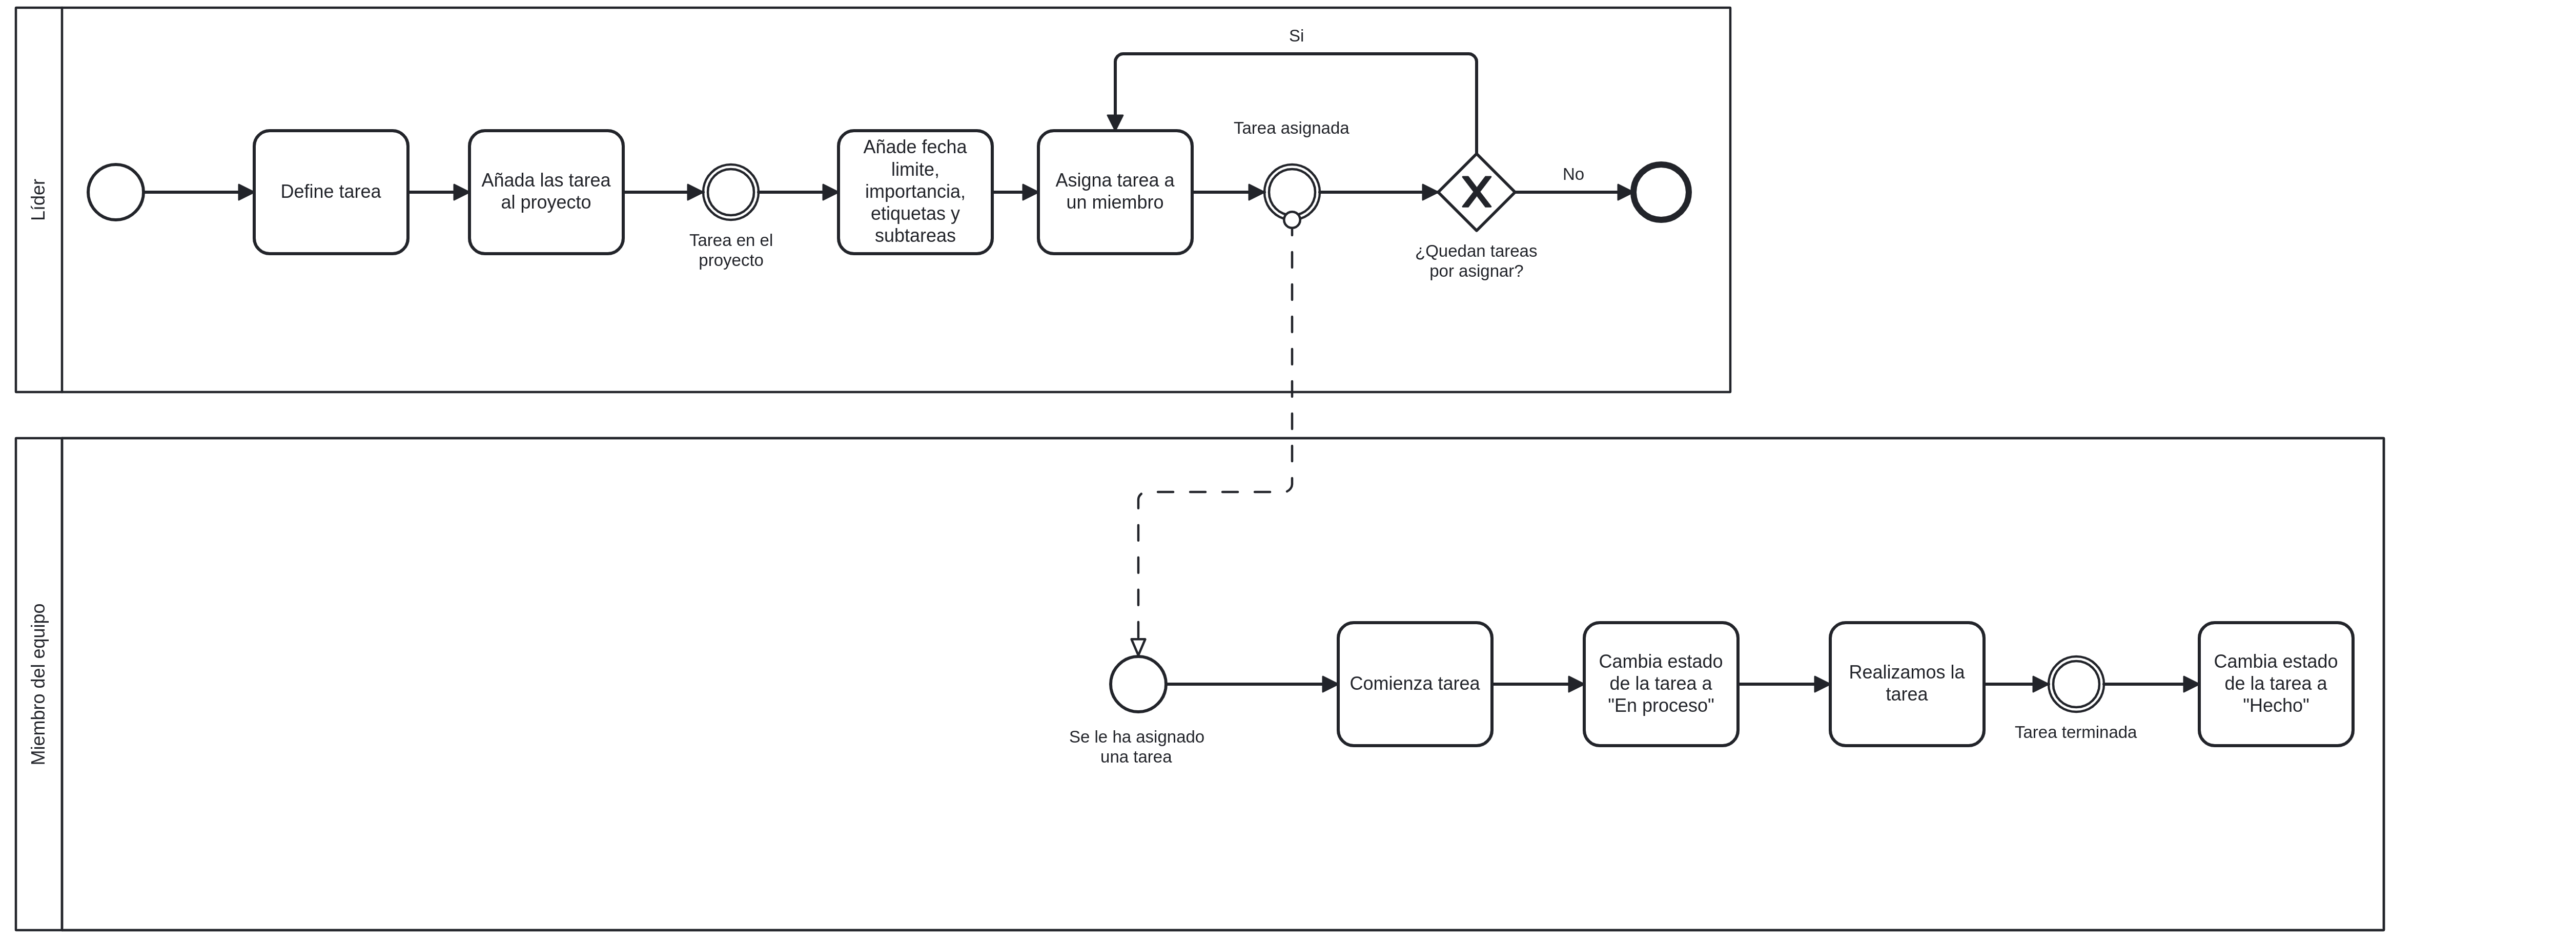
\includegraphics[width=1\linewidth]{ProjectsBPMN.png}
    \caption{Diagrama BPMN del flujo de trabajo de una empresa}
    \label{fig:BMMN_trabajo}
\end{figure}
\paragraph{}
Nuestro flujo de trabajo no ha sido como este; se basaba en cada día que hemos trabajado en el proyecto, lo primero que hacíamos era abrir este módulo y ver el estado global de este mediante la vista Kanban. Si en la columna \textit{En proceso} se encontraba alguna tarea, continuábamos con ella; si, por el contrario, estaba vacía, seleccionábamos una nueva tarea. En el momento en que hemos acabado con todas las tareas, hemos comenzado a realizar la memoria, tarea que en el tablero estaba bloqueada por el resto de tareas. Con este diagrama BPMN se refleja nuestro flujo.

\begin{figure}[h]
    \centering
    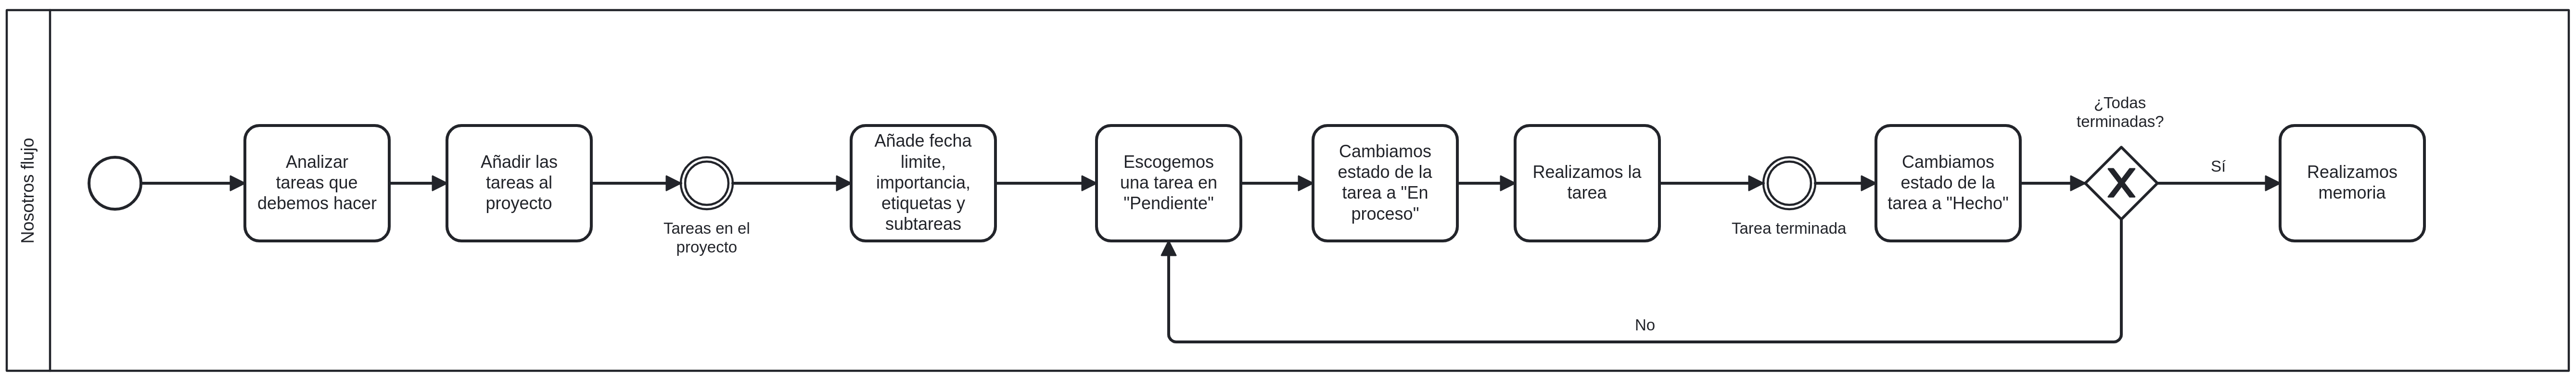
\includegraphics[width=1\linewidth]{ProjectsBPMN_2.png}
    \caption{Diagrama BPMN de nuestro flujo de trabajo}
\end{figure}
\paragraph{}
Bien es cierto que esta regla no se ha llevado a raja tabla, ya que ha habido ocasiones que había tareas en la segunda columna y escogíamos una nueva tarea. Estas decisiones siempre se han tomado de forma consensuada y fundamentada. Estas decisiones se han basado en bloqueos o porque las subtareas que faltaban eran para obtener la máxima nota.

\subsection{Conclusiones}
\paragraph{}
Tras haber trabajado con este módulo, consideramos que es uno de los mejores módulos que proporciona Odoo. Es intuitivo, fácil de usar y muy útil. Nos ha permitido llevar control en todo momento del estado de nuestro trabajo y saber qué tarea debíamos hacer en cada momento. Además, su vista Kanban permite cambiar el estado de las tareas de una forma cómoda y rápida. Esta vista se asemeja mucho a los tablones de tarjetas que se utilizan normalmente, permitiendo que desde cualquier lugar se pueda modificar y no sea necesario estar de forma presencial.
\paragraph{}
Creemos que no hemos llegado a exprimir todo su potencial al no haber utilizado la asignación de tareas. Realizando un análisis de nuestra organización en este proyecto, consideramos que podría haber sido mucho mejor, desde dividir las tareas a realizar el trabajo de forma más constante y no dejando gran parte de las tareas para las últimas semanas. Por último, ha habido tareas que se deberían haber realizado desde el principio como la instalación de Odoo en una máquina remota y la realización de backups diarias. Esto nos hubiera ahorrado muchos problemas y facilitado el trabajo.

\paragraph{}
En resumen, el módulo de gestión de proyectos de Odoo ha sido una herramienta invaluable para nuestro equipo, proporcionando una base sólida para la colaboración y el seguimiento del progreso del proyecto. Al reflexionar sobre nuestra experiencia, reconocemos las áreas de mejora y nos comprometemos a aplicar estas lecciones en proyectos futuros para lograr resultados aún más exitosos.
